\documentclass[12pt,a4paper,openany]{extarticle}
% подключаем собственный стилевой файл
\usepackage{mystyle}
\selectlanguage{russian}
\graphicspath{{./pictures/}}
\usepackage[pdftex]{lscape}
\usepackage{graphicx}
\usepackage{systeme}

\begin{document}
\part*{Лабораторная работа №3\\ Прямая и обратная задача кинематики. DH параметры.}
\section{Методические рекомендации}
\hspace*{\parindent}До начала работы студент должен выполнить предыдущие лабораторные этого цикла.

\section{Теоретические сведения}

\paragraph*{Параметры Денавита-Хартенберга\\}

\hspace*{\parindent}Как известно, для определения любого трехмерного тела в пространстве достаточно задать ему 6 координат (3 координаты перемещения и 3 координаты вращения). Для оптимизации задачи описания положения тела, существует метод, позволяющий сократить число необходимых координат до 4 - метод Денавита - Хартенберга.\\

\hspace*{\parindent}Координаты, позволяющие описать положение тела данным методом называются параметрами Денавита-Хартенберга:
\begin{enumerate} 
 \item[1.] Координатами $a_i$ - обозначаются расстояния по осям $x_i$ (текущая ось) от  $z_{i-1}$ до $z_i$;
 \item[2.] Координаты $\alpha_i$ - обозначают угол вращения оси $x_i$ (текущая ось) от  $z_{i-1}$ до $z_i$;
 \item[3.] Координатами $d_i$ - обозначаются расстояния по осям $z_{i-1}$ (предыдущая ось) от  $x_{i-1}$ до $x_i$;
 \item[4.] Координаты $\theta_i$ - обозначают угол вращения оси $z_{i-1}$ (предыдущая ось) от  $x_{i-1}$ до $x_i$.\\
 \end{enumerate}
 
 \paragraph*{Определение систем координат\\}
 
\hspace*{\parindent}Для удобного определения осей в каждом звене есть несколько правил:
\begin{enumerate} 
\item[1.] Ось $z_i$ выбирается как сонаправленная с осью вращения(движения) $i+1$ сочленения. Далее расположение смежных звеньев будет определяться именно положением этой оси.
\item[2.] Для оси $x_i$ существуют два условия: ось $x_i$ перпендикулярна оси $z_{i-1}$ и пересекает её при мысленном продолжении. (Для упрощения задачи желательно, чтобы в начальных(нулевых) конфигурациях оси $x_{i-1}$ и $x_i$ были сонаправлены.)
\item[3.] Ось $y_i$ задается согласно принципу правой тройки векторов, чтобы выполнялось тождество ($y_i = z_i x x_i$).
 \end{enumerate}

(КАРТИНКИ С ОСЯМИ)\\

\begin{center}
    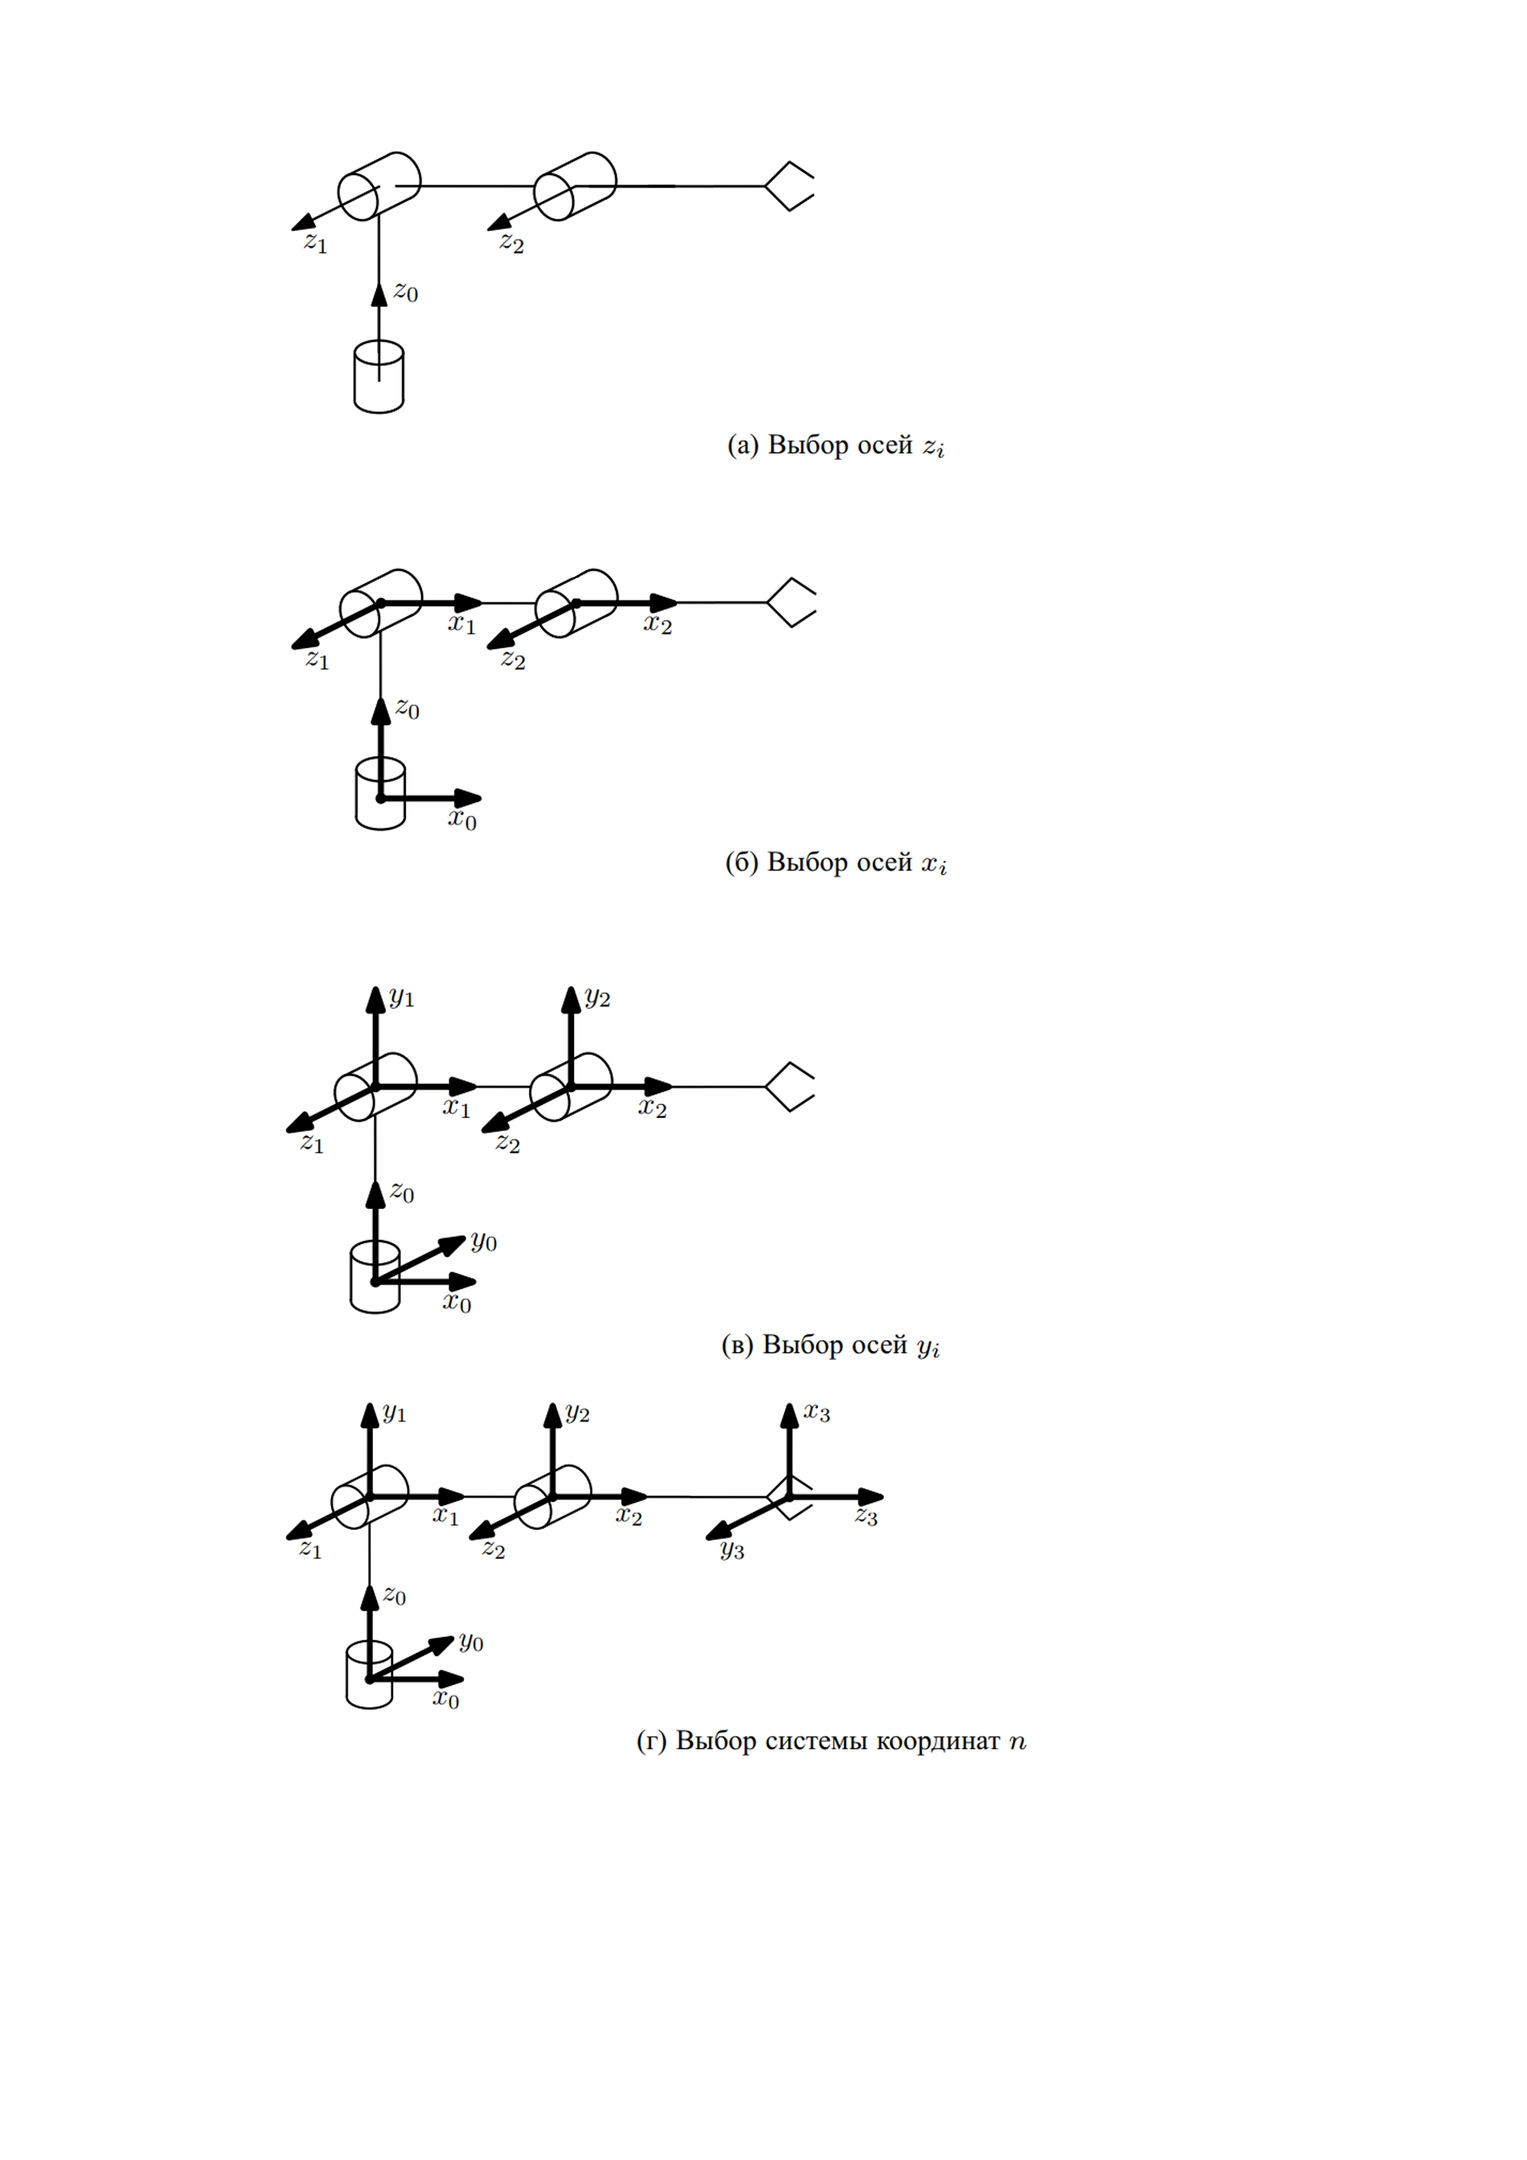
\includegraphics[width=\textwidth]{axes.jpg}\\
\end{center}

\hspace*{\parindent}Как ранее говорилось, вначале выбираются значения осей $z_i$: ось вращения первого звена будет проходить через ось изображаемого цилиндра, т.к. вращение происходит в этой плоскости, аналогично выбираются оси для остальных звеньев вращения, также можно заметить, что можно было выбрать направление осей $z_1$ и $z_2$ "от нас", но это  ухудшает наглядность схемы, поэтому выбирается направление "на нас". Оси $x_i$ выбираются по принципу перпендикулярности к соответствующим осям $z_i$, и направленные на пересечение с последующими из них, так выбрано направление "вправо" в первом звене и сонаправленном с ним втором для нулевого параметра начального угла в параметрах DH. Далее не происходит только смещение по оси перпендикулярной оси вращения, поэтому направление осей $x_i$ остаётся неизменным. Оси $y_i$ достраиваются в соответствии с правилом правой тройки векторов (можно использовать и левую, что приведёт к некотором изменениям знаков в дальнейших преобразованиях, но наиболее используемой является правая). Система последнего звена получается путём смещения на некоторое расстояние, поскольку схват и его сочленения статичны.\\
 
 \paragraph*{Практическая часть\\}
 
\hspace*{\parindent}Рассмотрим нахождение этих параметров на конкретной задаче:\\
(КАРТИНКИ С ПАРАМЕТРАМИ)\\

\hspace*{\parindent}После того, как были получены значения, достаточные для описания положения тела в пространстве, можно приступать к задачам нахождения связи между обобщенной системы координат манипулятора и системы координат, связанной со схватом (рабочим инструментом). Для этого будут использованы матричные преобразования систем координат.\\

 
\paragraph*{2.2 Прямая задача кинематики}$\phantom{-}$\\
\hspace*{\parindent} Прямая задача кинематики (ПЗК) заключается в вычислении координат системы, связанной со схватом (рабочим инструментом), в зависимости от обобщенных координат манипулятора.\\
\hspace*{\parindent}Для решения ПЗК рассматриваются две системы координат: исходная, связанная с «землей» $o_0 x_0 y_0 z_0$ и итоговая, связанная с рабочим инструментом $o_n x_n y_n z_n$. Как известно, расположение этих двух систем друг относительно друга определяется тремя линейными и тремя угловыми координатами.\\
\hspace*{\parindent}Итак, рассмотрим подробнее переход между обобщенными и глобальными координатами. Данный переход можно представить в виде: $k^0 = T_n^0 k^n$, 

где $T_n^0$ - матрица преобразования, несущая информацию о линейном смещении и пространственной ориентации одной системы относительно другой.\\


\begin{equation*}\label{eq:model}
T_n^0=
    \begin{bmatrix}
    n_x & s_x & a_x & p_x \\
    n_y & s_y & a_y & p_y \\
    n_z & s_z & a_z & p_z \\
    0 & 0 & 0 & 1 \\
    \end{bmatrix}
    =
     \begin{bmatrix}
    n_n^0  &  s_n^0 & a_n^0 & p_n^0 \\
    0 & 0 & 0 & 1\\
    \end{bmatrix}
     =
     \begin{bmatrix}
    R_n^0  &  p_n^0 \\
     0 & 1\\
    \end{bmatrix}
    ,\\
\end{equation*} 

\hspace*{\parindent} где векторы  $n_n^0$,  $s_n^0$ и $a_n^0$ выражают направления осей $x_n$, $y_n$ и $z_n$, О O соответственно, относительно системы координат $o_0 x_0 y_0 z_0$, $R_n^0 \in$ SO - матрица 3х3 вращения системы  $o_n x_n y_n z_n$ относительно $o_0 x_0 y_0 z_0$, $p_n^0$ $\in$ $R^3$ - вектор линейного смещения начала координат системы  $o_n x_n y_n z_n$ относительно $o_0 x_0 y_0 z_0$.\\
\hspace*{\parindent} матрица $T_n^0$ имеет размерность 4х4, значит нужно расширить векторы координат $v^0$ и $v^n$ единицей для соответствия размерностей в матричных уравнениях:\\
\begin{equation*}\label{eq:model}
     \begin{bmatrix}
     x^0 \\
     y^0\\
     z^0\\
     1\\
    \end{bmatrix}
     =T_n^0
     \begin{bmatrix}
     x^n \\
     y^n\\
     z^n\\
     1\\
    \end{bmatrix}
    .\\
\end{equation*} 
\hspace*{\parindent} Рассмотрим самые важные свойства, характеристики и отдельные элементарные компоненты, которые будут активно использоваться в пособии:\\

1. Поворот на нулевой угол определяется единичной матрицей\\
\begin{equation*}\label{eq:model}
R_{\beta=0} = 
     \begin{bmatrix}
    1 & 0 & 0\\
    0 & 1 & 0\\
    0 & 0 & 1\\
    \end{bmatrix}
     =I
\end{equation*} 

2. Поворот в отрицательном направлении определяется
\begin{equation*}\label{eq:model}
R_{-\beta} = R_{\beta}^{-1} = R_{-\beta}^T
\end{equation*} 

3. Существуют так называемые базовые матрицы вращения вокруг осей x, y и z:
\begin{equation*}\label{eq:model}
R_{x, \beta} = 
     \begin{bmatrix}
    1 & 0 & 0\\
    0 & cos\beta & -sin\beta\\
    0 & sin\beta & cos\beta\\
    \end{bmatrix}
    , \\
\end{equation*} 

\begin{equation*}\label{eq:model}
R_{y, \beta} = 
     \begin{bmatrix}
    cos\beta & 0 & sin\beta\\
    0 & 1 & 0\\
    -sin\beta & 0 & cos\beta\\
    \end{bmatrix}
    , \\
\end{equation*} 

\begin{equation*}\label{eq:model}
R_{z, \beta} = 
     \begin{bmatrix}
   
    cos\beta & -sin\beta & 0\\
    sin\beta & cos\beta & 0\\
    0 & 0 & 1\\
    \end{bmatrix}
    , \\
\end{equation*} 
где $\beta$ - некоторый угол.\\

\begin{center}
    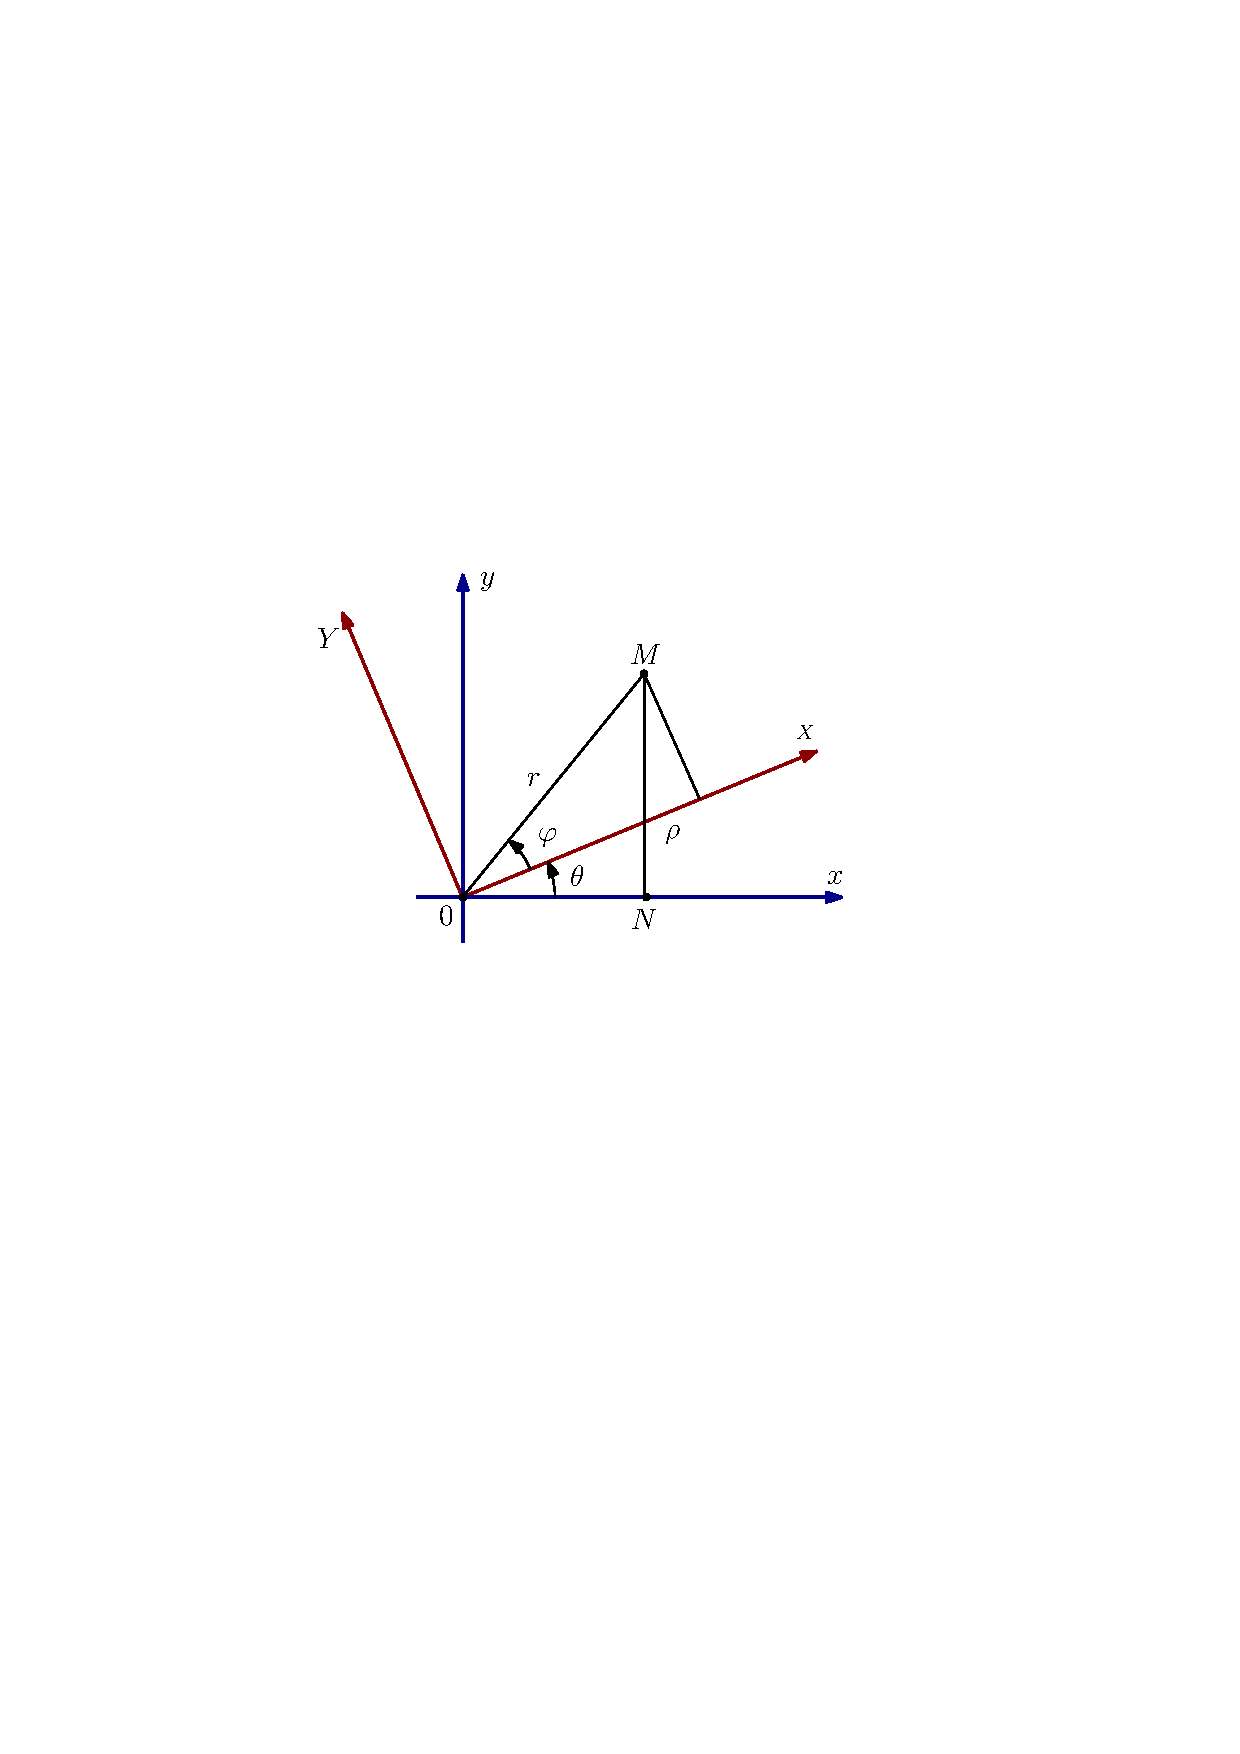
\includegraphics[width=0.7\textwidth]{Lab3/pictures/rotation.pdf}\\
    Рисунок 2.2.1 Старая система и новая системы координат\\
\end{center}
\hspace*{\parindent} Рассмотрим две системы координат, заданные на плоскости, с общим началом в точке О: исходная система Oxy и новая OXY, которая повёрнута на угол между осями Ox и OX, равный $\theta$ (угол между осями Oy и OY также равен $\theta$). Выведем формулы, которые выражают старые координаты x и y точки М, выбранной произвольным образом, через ее новые координаты X и Y.\\
Для этого перейдем в полярные координаты: у старой системы координат полярная ось совпадает с Ox, а у новой - с OX. Пусть у точки М в новой полярной системе координат будет полярный угол $\phi$ и полярный радиус r. Тогда, в старой полярной системе полярный угол точки М= $\phi+\theta$, а радиус останется тем же.\\
Таким образом: \\
$x=rcos(\theta+\phi)$,\\
$y=rsin(\theta+\phi)$.\\
С использованием тригонометрических тождеств и суммы двух углов, получаем:\\
$x=r(cos\theta cos\phi - sin \theta sin \phi) = (rcos \phi)cos \theta - (rsin\phi)sin\theta$\\
$y=r(sin\theta cos\phi + cos \theta sin\phi) = (rcos\phi)sin\theta + (rsin\phi)cos\theta$\\
Т.к. $rcos\phi$ = X и $rsin\phi$ = Y, получаем:\\
\begin{equation*}
 \begin{cases}
x=Xcos\theta - Ysin\theta,\\
y=Xsin\theta + Ycos\theta.\\
 \end{cases}
\end{equation*}
или\\
\begin{equation*}\label{eq:model}
R_{z, \theta} = 
     \begin{bmatrix}
       cos\theta & -sin\theta \\
    sin\theta & cos\theta \\
      \end{bmatrix}
    , \\
\end{equation*} \\

\hspace*{\parindent} Возвращаясь к методу Денавита-Хартенберга, напомним, что на предыдущем шаге были получены по четыре параметра для каждого звена манипулятора. Теперь из них необходимо построить соответствующие матрицы однородного преобразования следующим способом:\\
%
\begin{equation*}\label{eq:model}
T_i^{i-1} = T_{z,{\theta_i}} T_{z,{d_i}} T_{x,{a_i}} T_{z,{\alpha_i}} = \\
     \begin{bmatrix}
      R_{z,{\theta_i}} & 0\\
      0 & 1 \\
    \end{bmatrix}
    \begin{bmatrix}
      I & p_{d_i}\\
      0 & 1 \\
    \end{bmatrix}
    \begin{bmatrix}
      I & p_{\alpha_i}\\
      0 & 1 \\
    \end{bmatrix}
    \begin{bmatrix}
      1 & 0\\
      0 & R_{x,{\alpha_i}} \\
    \end{bmatrix}
    = \\
     \begin{bmatrix}
      c_{\theta_i} & -s_{\theta_i}c_{\alpha_i} & s_{\theta_i}s_{\alpha_i} & \alpha_i c_{\theta_i} \\
      s_{\theta_i} & c_{\theta_i}c_{\alpha_i} & -c_{\theta_i}s_{\alpha_i} & \alpha_i s_{\theta_i} \\
      0 & s_{\alpha_i} & c_{\alpha_i} & d_i\\
      0 & 0 & 0 & 1\\
    \end{bmatrix}
    ,\\
\end{equation*} 
\hspace*{\parindent}где i - номер звена,  $R_{z,{\theta_i}}$ и $R_{x,{\alpha_i}}$  - базовые матрицы вращения (см. свойство №3):
\begin{equation*}\label{eq:model}
R_{z, \theta_i} = 
     \begin{bmatrix}
    cos\theta_i & -sin\theta_i & 0\\
    sin\theta_i & cos\theta_i & 0\\
    0 & 0 & 1\\
    \end{bmatrix}
    , \\
\end{equation*} 

\begin{equation*}\label{eq:model}
R_{x, \alpha_i} = 
     \begin{bmatrix}
    1 & 0 & 0\\
    0 & cos\alpha_i & -sin\alpha_i\\
    0 & sin\alpha_i & cos\alpha_i\\
    \end{bmatrix}
    , \\
\end{equation*} 
\hspace*{\parindent}где  $p_{d_i}$ и $p_{a_i}$ - векторы с ненулевыми компонентами $p_z= d_i$ и $p_x= a_i$, соответственно:

\begin{equation*}\label{eq:model}
 p_{d_i} = 
     \begin{bmatrix}
   0\\
   0\\
   d_i\\
    \end{bmatrix}
, p_{a_i} =
     \begin{bmatrix}
   a_i\\
   0\\
   0\\
    \end{bmatrix}
\end{equation*}

\hspace*{\parindent}Итоговую матрицу, связывающую все системы координат, как и в случае с матрицами вращения, можно получить последовательным перемножением:\\

\begin{equation*}\label{eq:model}
T_n^0(q) = T_1(q)T_2(q)..T_n(q) = 
     \begin{bmatrix}
    R_n^0(q) & p_n^0(q)\\
    0 & 1\\
    \end{bmatrix}
    ,
\end{equation*} 
\hspace*{\parindent}где матрица вращения  $R_n^0(q)$ и вектор $p_n^0(q)$ задают, соответственно, ориентацию и положение системы координат, связанной со схватом или рабочим инструментом, относительно базовой системы в зависимости от конфигурации манипулятора, заданной вектором обобщенных координат $q \in \mathbb {R}^n$
\paragraph*{2.3 Обратная задача кинематики}$\phantom{-}$\\
\hspace*{\parindent}Обратная задача кинематики (или обобщенно ОЗК) заключается в определение обобщенных координат через линейные и угловые координаты рабочего инструмента (хвата). \\

\hspace*{\parindent}Рассмотрим аналитический (геометрический) метод расчёта обобщенных коэффициентов системы:\\
\begin{enumerate} 
\item[1.]  В начале рассмотрим схему, которая была получена после присвоения каждому звену системы координат и определения углов вращения каждого из них\\

\begin{center}
    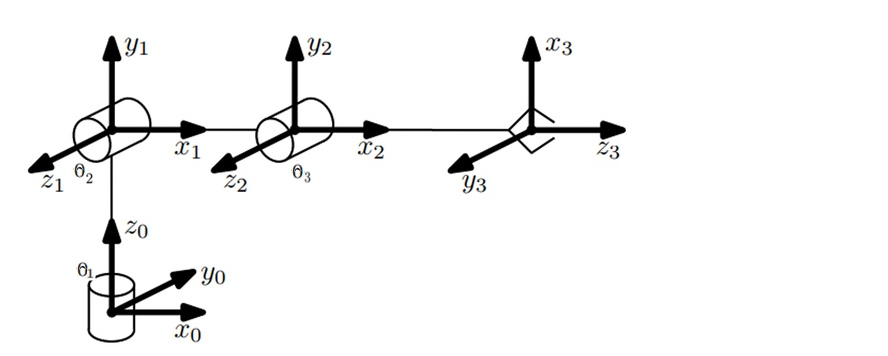
\includegraphics[width=0.9\textwidth]{axesIK.jpg}\\
    Рисунок 2.3.1 схема манипулятора с обозначенными осями и углами вращений.\\
\end{center}

\item[2.] Далее рассмотрим вид сверху для данной системы\\

\begin{center}
    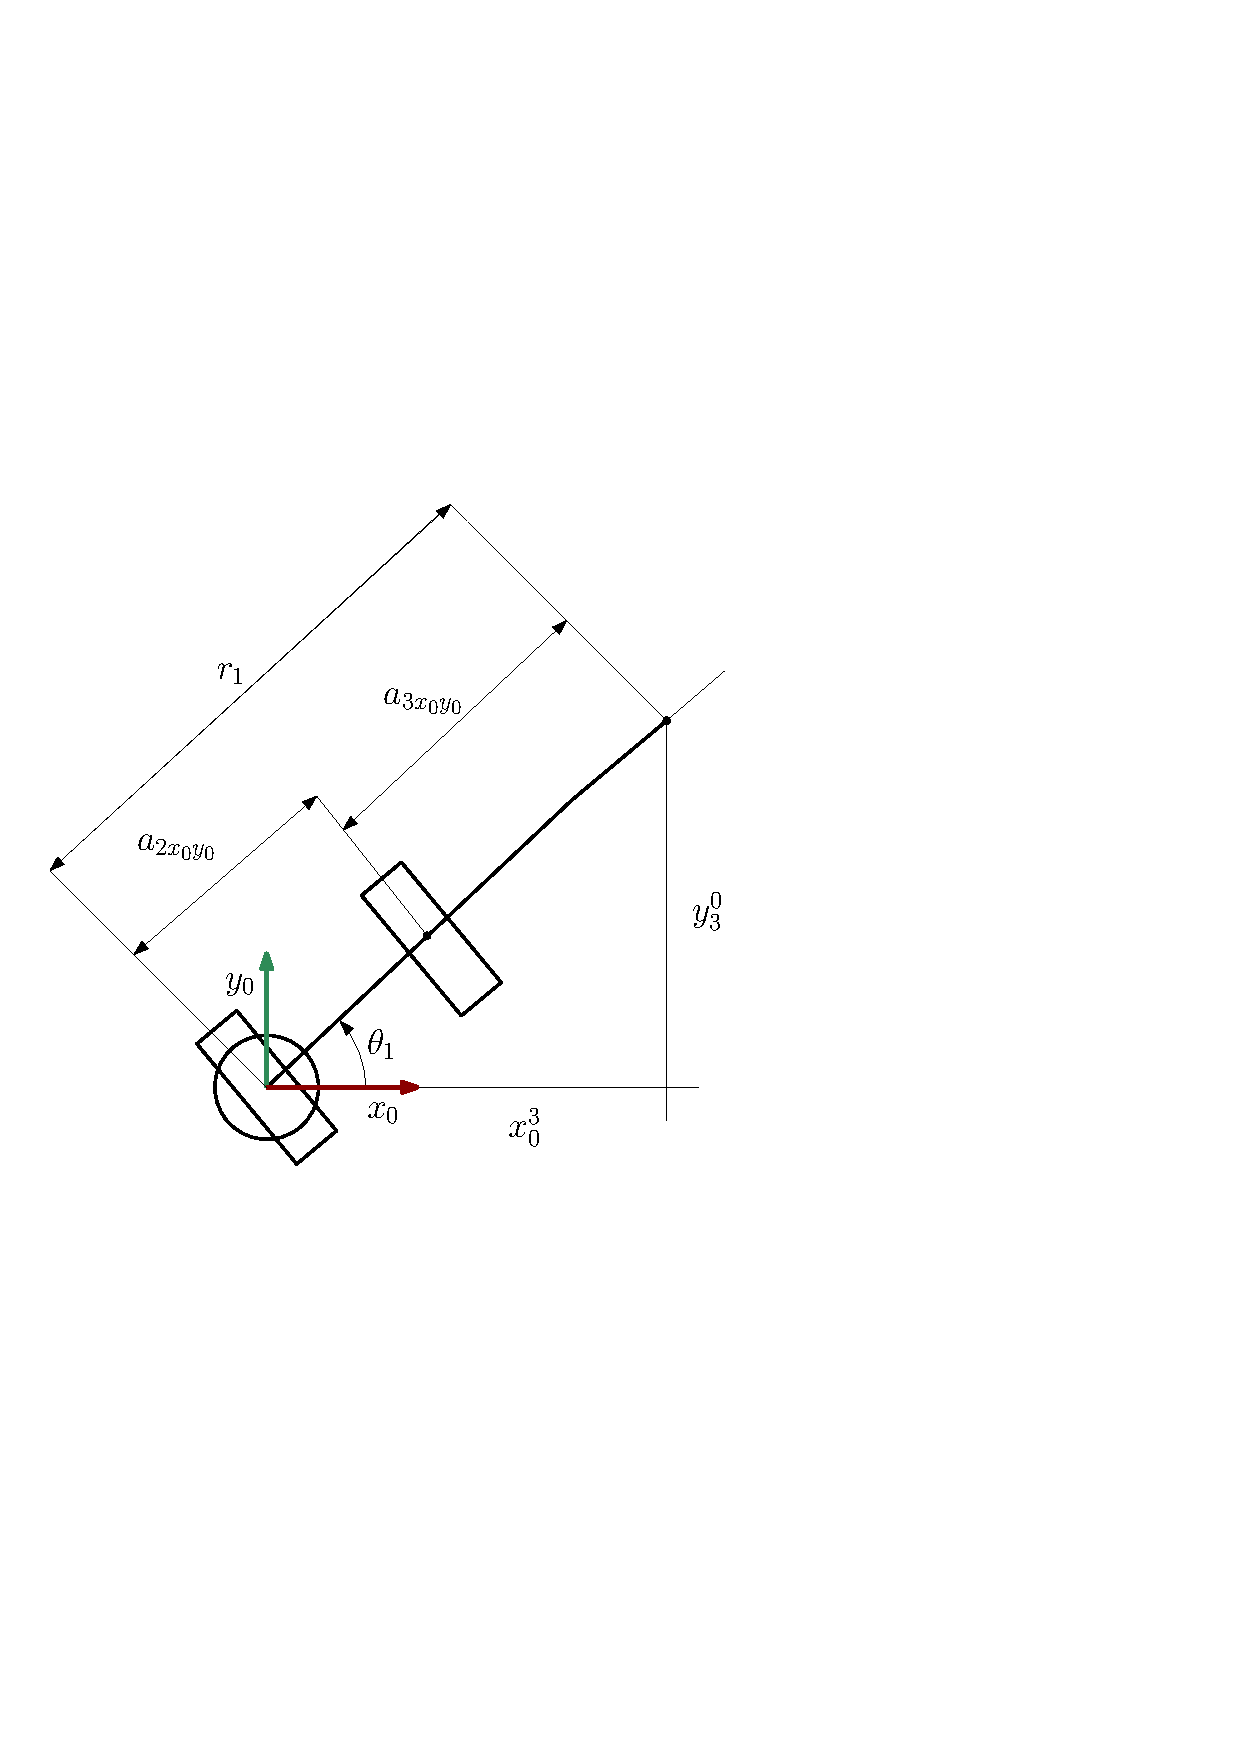
\includegraphics[width=0.5\textwidth]{2.pdf}\\
     Рисунок 2.3.2 Вид схемы сверху (проекция $x_0 y_0$).\\
\end{center}


Обозначим нулевую систему координат и угол вращения $\theta_1$ (можно было бы ещё обозначить известные параметры $a_2$ и  $a_3$, но в данной проекции отображаются $но в данном случае мы наблюдаем лишь их проекции. (мне кажется больше в скобках ничего не нужно)$не явные(известные) значения этих параметров, а их проекции на плоскость $x_0 y_0$, которые соответственно изменяются с изменениями угла, поэтому не указываются на таком виде). Можно заметить, что искомый угол $\theta_1$ выражается через отношение $y_3^0$ $x_3^0$:\\

\begin{equation}
    \theta_1=arctg(\frac{y_3^0}{x_3^0});
\end{equation}


\item[3.] Далее рассмотрим вид спереди данной системы, придав звеньям некоторое смещение $Не уверен, но мне кажется что комментарии не нужны$(для более наглядного выражения углов). Тут можно выделить неоднозначность решения ОЗК, поскольку можно заметить, что прийти в данную точку возможно несколькими вариантами смещения, к примеру:\\

\begin{center}
    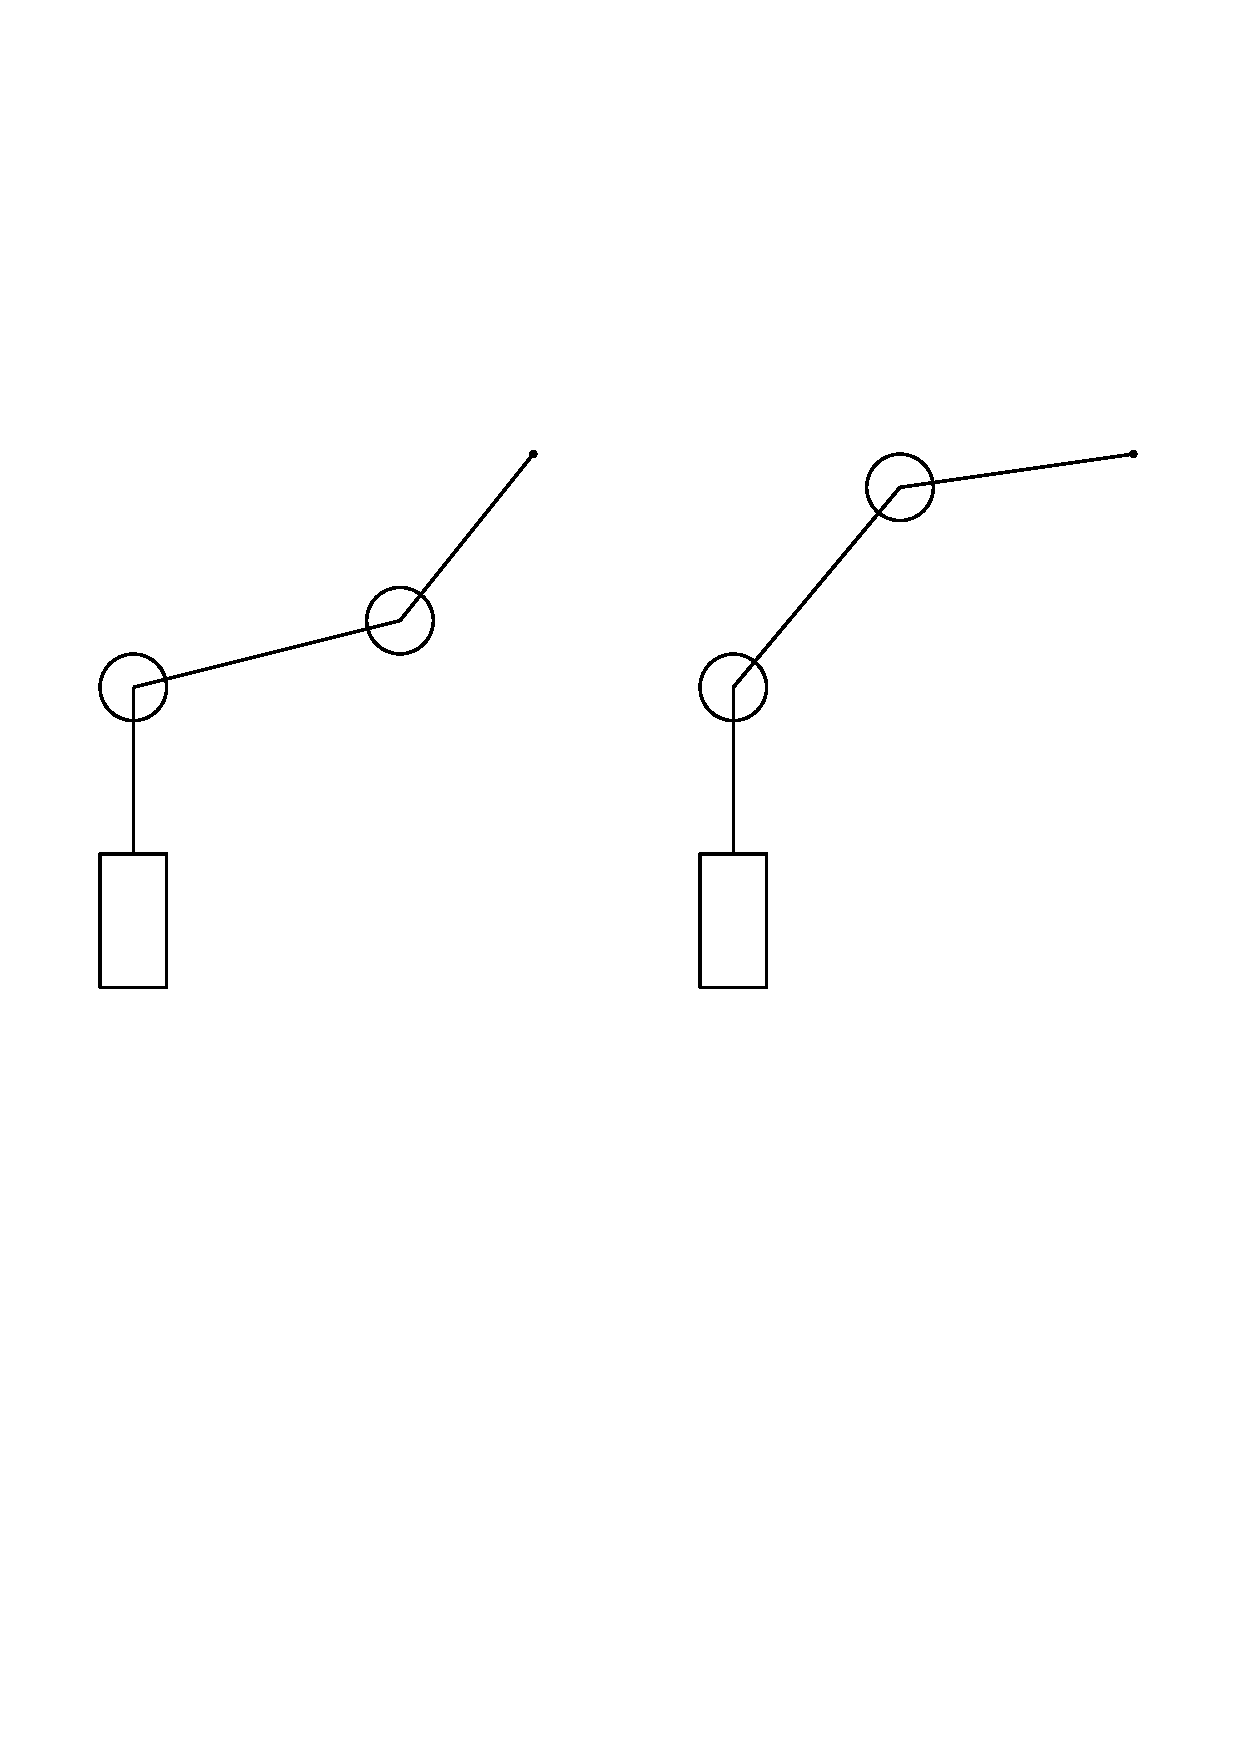
\includegraphics[width=0.55\textwidth]{1.pdf}\\
    а) Второе сочленение расположено снизу    б) Второе сочленение расположено сверху.\\
     Рисунок 2.3.3 схема манипулятора для некоторых одинаковых коэффициентов рабочего инструмента.%не оч догоняю решение этой проблемы, но частично понимаю, что имеет ввиду Дима\\
     $Рисунок 2.3.3 схема манипулятора для некоторых одинаковых коэффициентов рабочего инструмента.а) Второе сочленение расположено снизу, б) второе сочленение расположено сверху\\$%Вроде обычно так обозначают, либо в данном случае можно вообще без объяснения, если кратко то я могу ещё попридираться к этому
\end{center}
%Каждая конфигурация при решении ОЗК ограничивает рабочую облась, поэтому при решении задачи отдается предпочтение конфигурации которая в большей степени удовлетворяет достижению необходимой нам рабочей области.
Для примера будет рассматриваться вариант с верхним расположением второго сочленения. Потому что каждая конфигурация при решении ОЗК ограничивает некоторую рабочую область, поэтому при выборе конфигурации отдается предпочтение той, которая в большей степени удовлетворяет достижению необходимой рабочей области. %тут появился Димин текст, если что \\
Итак, здесь помимо обозначения нулевой системы координат (можем обозначить только $z_1$, поскольку она является единственной не перпендикулярной осью вращения и задает своё изменение для $x_0$ и $y_0$) и углов вращения: $\theta_2$,  $\theta_3$ - можно обозначить параметры $d_1$, $a_2$ и $a_3$, поскольку их величины в данной проекции не изменяются. Также можно задать вспомогательные величины углов и длин: соединение первого и третьего сочленения $r_3$, достроение до треугольника $r_1$ и $r_2$, а также углы $\phi_1$, $\phi_2$, $\phi_3$. %убрались пара уточнений \\
%Мне кажется слишком много отступлений в скобочках, возможно я сейчас невыспавшийся злой и придираюсь, но я теряю мысль пока читаю отступления.

\begin{center}
    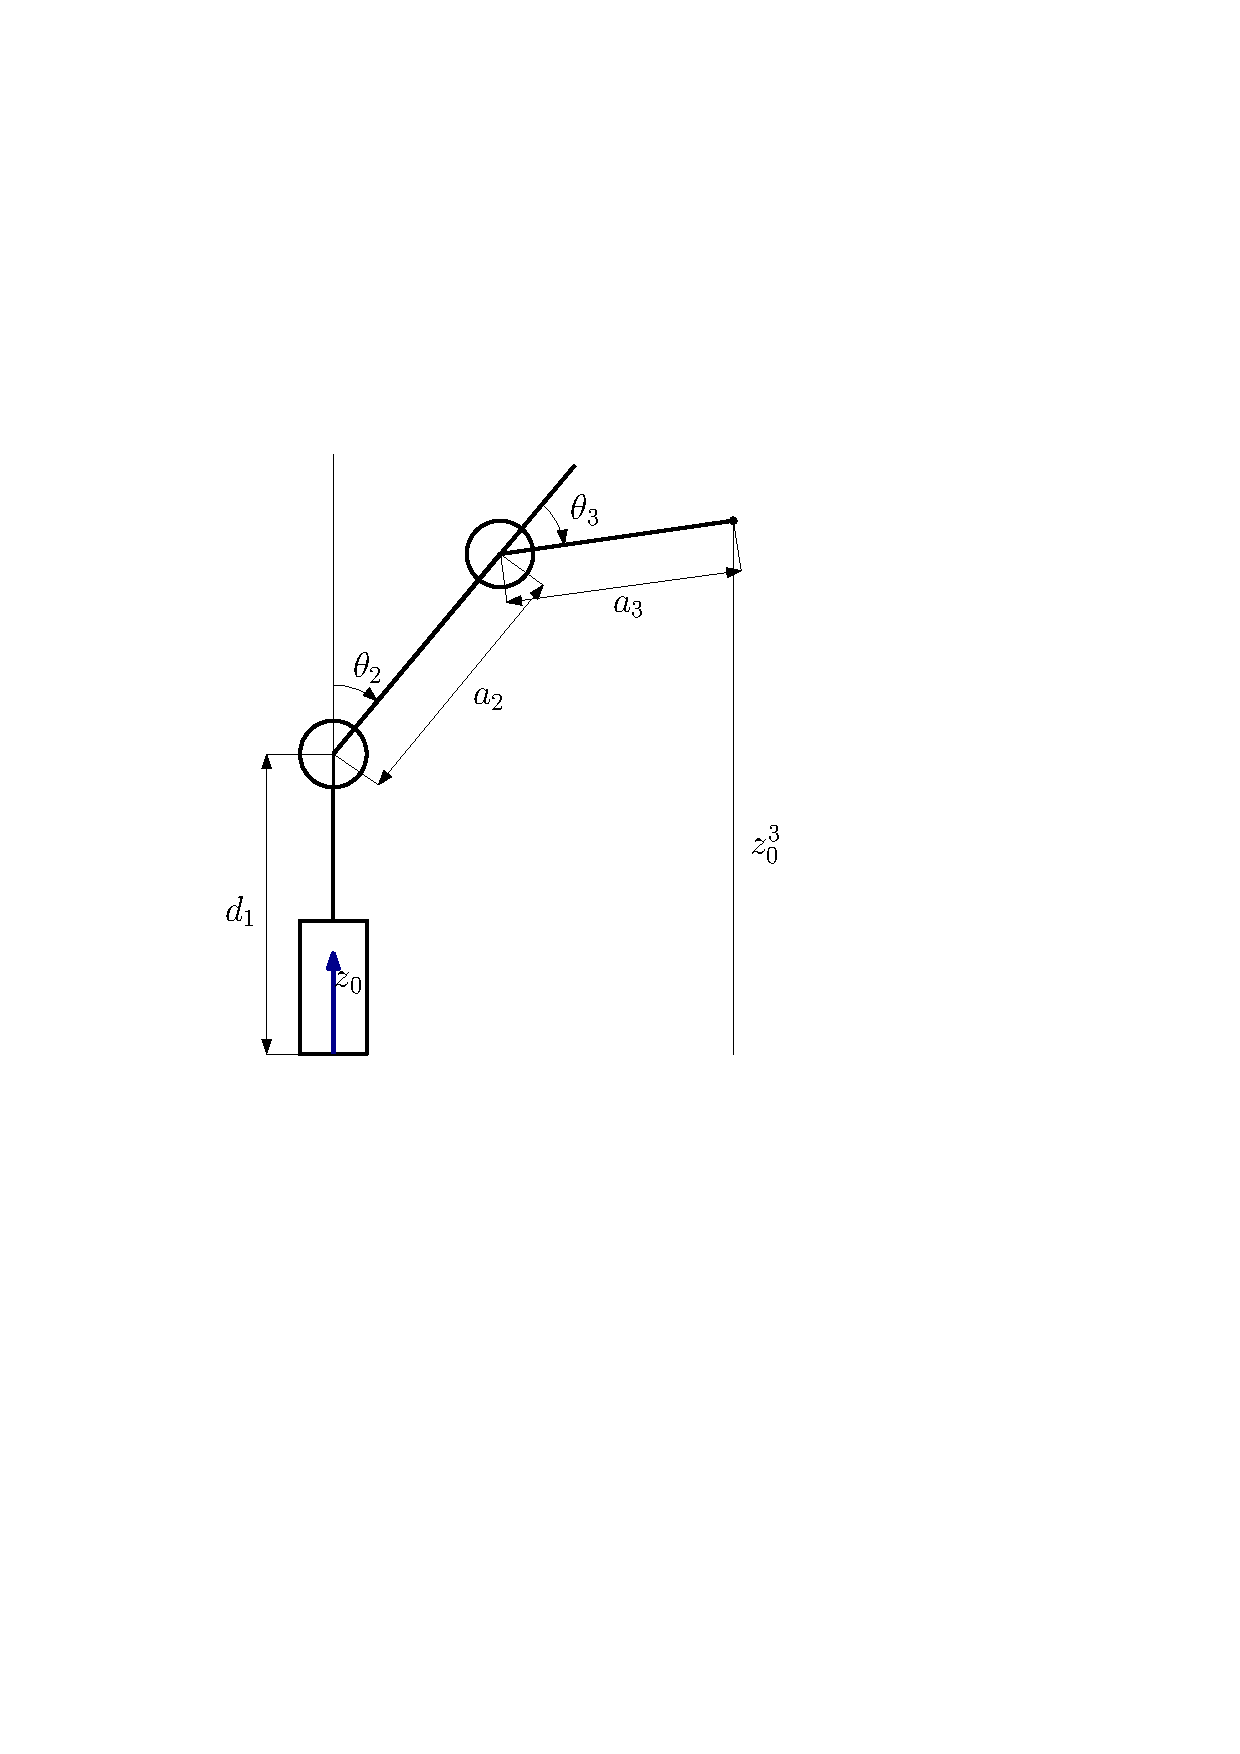
\includegraphics[width=0.4\textwidth]{3.pdf}\\
     Рисунок 2.3.4 Вид схемы спереди (проекция $x_0z_0$).\\
\end{center}

Рассмотрим поподробнее схему между вторым, третьим и инструментальным звеньями.\\

\begin{center}
    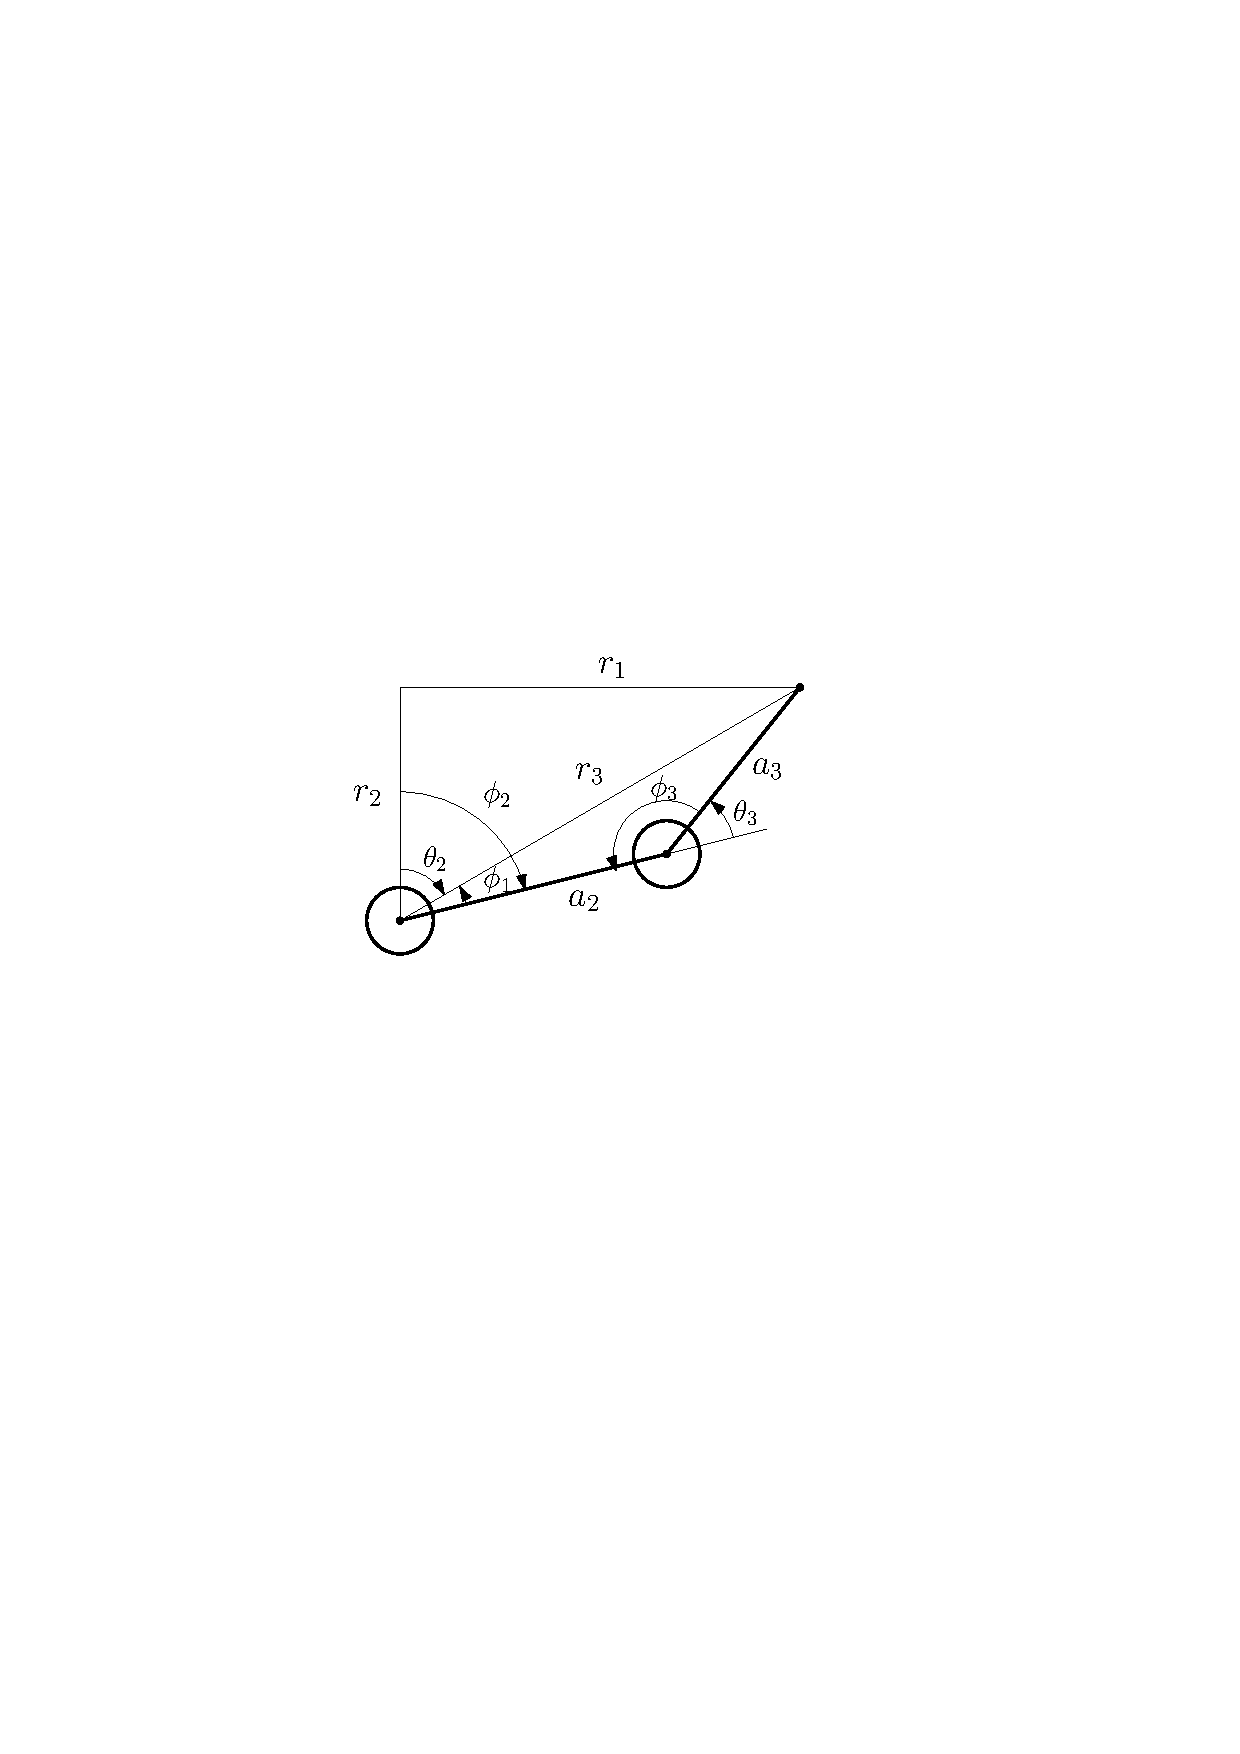
\includegraphics[width=0.5\textwidth]{4.pdf}\\
         Рисунок 2.3.5 Приближенное изображение схемы с необходимыми обозначениями. \\

\end{center}

Можно представить угол $\theta_2$ как разницу между углами $\phi_2$ и $\phi_1$:\\

\begin{equation}
    \theta_2 = \phi_2 - \phi_1;
\end{equation}

- где $\phi_2$ видно из рисунка (треугольник, образованный сторонами $r_1$, $r_2$ и $r_3$ прямоугольный, $\phi_2$ определяет отношение катетов);

\begin{equation}
    \phi_2 = arctg(\frac{r_1}{r_2});
\end{equation}

- $r_2$ находится как разность между $z_0^3$ и $d_1$: \\
$$r_2=z_3^0 - d_1$$
- $r_1$ определяется из предыдущей проекции ($x_0y_0$) как сумма проекций $a_{2x0y0}$ $a_{3x0y0}$, которые в свою очередь определяются через теорему Пифагора:\\ $$r_1=a_{2x0y0}+a_{3x0y0}=\sqrt{(x_3^0)^2+(y_3^0)^2}$$
- $\phi_1$ находим через теорему косинусов в треугольнике, образованном сторонами $a_2$, $a_3$, $r_3$:\\
$$a_3^2 = a_2^2 + r_3^2 - 2 a_2 r_3 cos\phi_1$$
$$cos\phi_1 = \frac{a_2^2 + r_3^2 - a_3^2}{2 a_2 r_3} $$

\begin{equation}
    \rightarrow \phi_1 = arccos(\frac{a_2^2 + r_3^2 - a_3^2}{2 a_2 r_3});
\end{equation}

- $r_3$ находится так же по теореме Пифагора:\\
%Вставить обозначения векторов
$$r_3=\sqrt{r_1^2+r_2^2}=\sqrt{(x_3^0)^2+(y_3^0)^2)+(z_3^0 - d_1)^2}$$
Таким образом получаем:\\

\begin{equation}
    \theta_2=arctg(\frac{r_1}{r_2}) - arccos(\frac{a_2^2 + r_3^2 - a_3^2}{2 a_2 r_3});
\end{equation}

\begin{equation}
    \theta_2=arctg(\frac{\sqrt{(x_3^0)^2+(y_3^0)^2}}{z_3^0-d_1}) - arccos(\frac{a_2^2 + ((x_3^0)^2+(y_3^0)^2)+(z_3^0 - d_1)^2) - a_3^2}{2 a_2 \sqrt{(x_3^0)^2+(y_3^0)^2)+(z_3^0 - d_1)^2}});
\end{equation}

Далее рассмотрим нахождение угла $\theta_3$, из рисунка 2.3.5 видно:

\begin{equation}
    \theta_3=180-\phi_3;
\end{equation}

Далее через теорему косинусов в треугольнике ($a_2$, $a_3$, $r_3$) определяется угол $\phi_3$:\\
$$r_3^2=a_2^2+a_3^2 - 2cos\phi_3 a_2 r_3 $$

\begin{equation}
    \phi_3 = arccos(\frac{a_2^2 + a_3^2 -r_3^2}{2a_2 r_3});
\end{equation}

\begin{equation}
    \theta_3=180-arccos(\frac{a_2^2 + a_3^2 -r_3^2}{2a_2 r_3})=;
\end{equation}

Подставляя в () значение $r_3$ получается:\\

\begin{equation}
    \theta_3 = 180-arccos(\frac{a_2^2 + a_3^2 -((x_3^0)^2+(y_3^0)^2)+(z_3^0 - d_1)^2)}{2a_2 \sqrt{(x_3^0)^2+(y_3^0)^2)+(z_3^0 - d_1)^2}});
\end{equation}

 \end{enumerate}

\section{Практическое задание}
\paragraph*{3.1 Описание практической части\\}

\hspace*{\parindent}Практическая часть лабораторной работы состоит из нескольких задач:\\

\begin{enumerate} 
\item[1.] Прочитать и постараться понять предложенный теоретический материал, представленный выше.
\item[2.] Собрать робот-манипулятор из наборов \textit{LEGO}.
\item[3.] Измерить и рассчитать для него параметры Денавита - Хартенберга.
\item[4.] По полученным параметрам расписать ПЗК системы.
\item[5.] А также ОЗК системы.
\item[6.] Проверить правильность своих расчетов посредством подстановки прямой и обратной задач в пакете \textit{Scilab}.
\item[7.] Написать программу, позволяющею по входным параметрам (координатам в обобщенной системе) перемещать рабочий инструмент (хват) в заданное положение и определять свои параметры в текущий момент (углы вращения по входным координатам)
\item[8.] Написать программу, позволяющею по входным параметрам (углам вращения) перемещать рабочий инструмент (хват) в заданное положение и определять свои параметры в текущий момент (координаты обобщенной системы по входным углам вращения).
\item[9.] Также в пакете \textit{Scilab} построить траектории движения и сравнить с имеющийся на готовом роботе. 
 \end{enumerate}

\section{Приложение А}
 \paragraph*{Пример\\}
 
\hspace*{\parindent}Рассмотрим нахождение DH параметров на конкретной задаче:\\

Пусть имеется такая система:\\
\begin{center}
    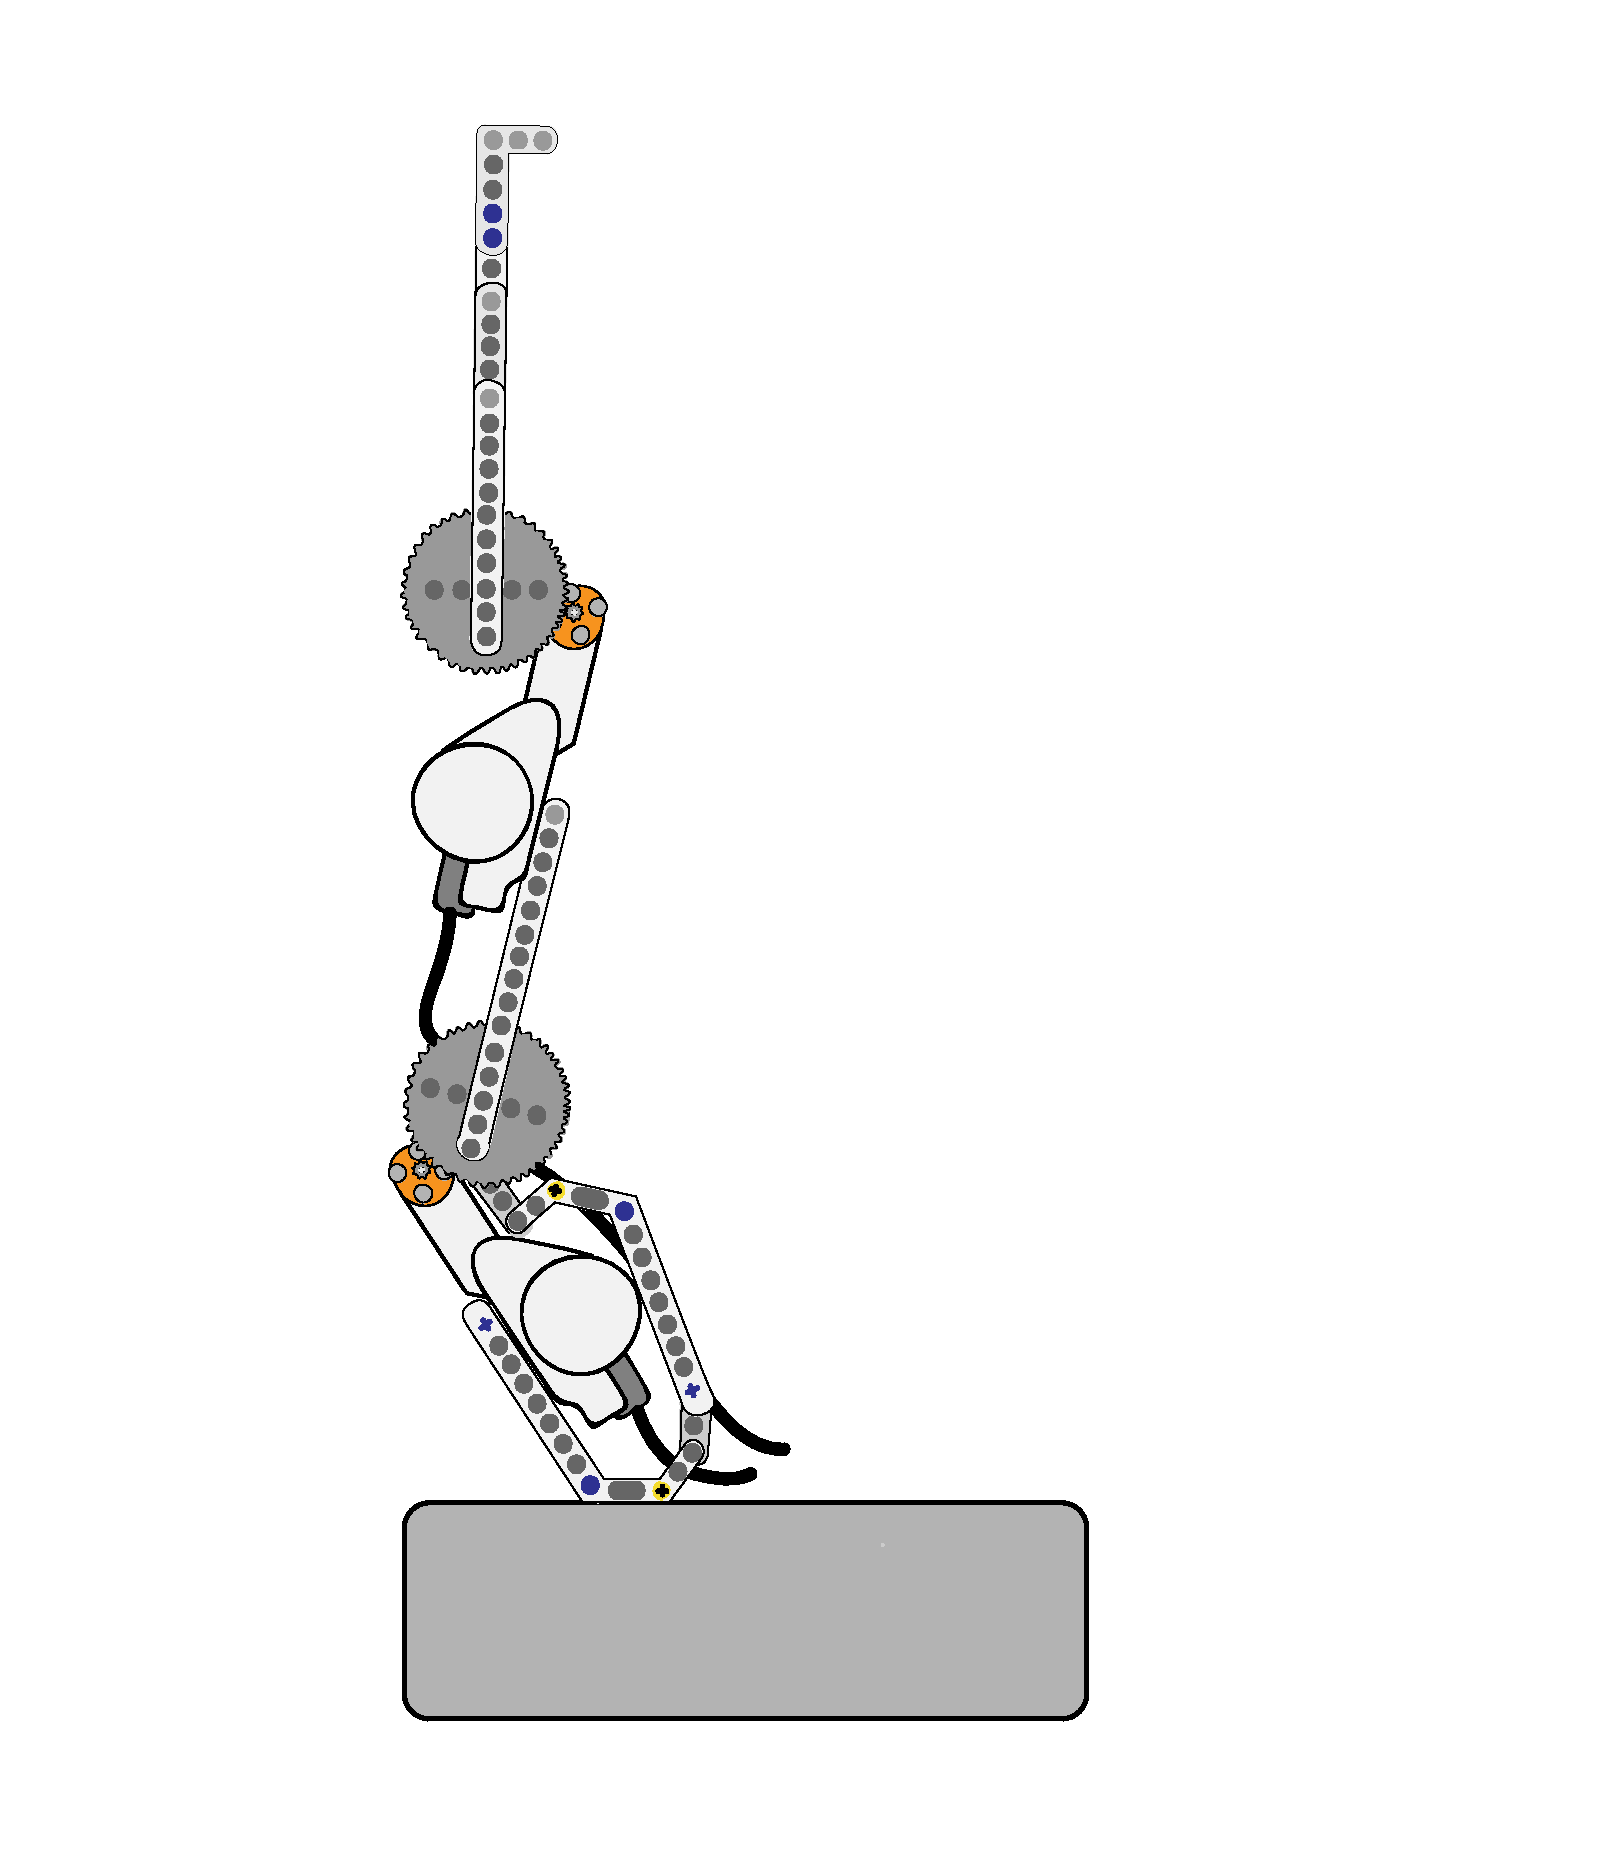
\includegraphics[width=0.6\textwidth]{DH1.pdf}\\
    Рисунок 2.1.2 Система для определения DH параметров.\\
\end{center}


\hspace*{\parindent}Расставляются положения DH-параметров по правилам, описанным выше:\\ 
\hspace*{\parindent}В начале определяются параметры $a_i$: системы $x_0y_0z_0$ и $x_1y_1z_1$ совпадают, следовательно сдвигов нет, далее рассматривается пара систем $x_1y_1z_1$ и $x_2y_2z_2$ здесь ость $z_2$ лежит в плоскости перпендикулярной рассматриваемому виду и располагается в направлении "от нас", её нулевая координата соответственно совпадает с нулевыми координатами $x_2$ и $y_2$, а значит $a_1$ определяется как расстояние от пересечения $x_1z_1$ до  $x_2y_2$ по оси $x_2$, следующее смещение между осями $z_2$ $z_3$ и $z_3$ $z_4$ выполняется аналогично, они направлены "от нас" и лежат в перпендикулярной плоскости, их начала лежат на пересечении двух других осей, соответственно получаются значения $a_2$ и $a_3$.\\
\hspace*{\parindent}Далее коэффициенты смещения $d_i$: имеется только смещение $d_1$ (поскольку остальные системы по осям $z_i$ не имеют сдвигов) от первой системы до второй.\\
Углы $\alpha_i$ определяются как поворот текущей оси $x_i$ от оси $z_{i-1}$ до оси $z_{i}$. Например, для первого звена ось $z_0$ направлена вверх, а $z_1$ от нас. Значит, поворот был на угол $\frac{\pi}{2}$. \\
\hspace*{\parindent}Углы $\theta_i$ определяются как углы вращения на сочленениях: можно заметить, что при переходе от первой системы ко второй производится дополнительный поворот на угол $\frac{\pi}{2}$, что также заносится в параметр, остальные углы подобного дополнительного вращения не имеют.\\
\begin{center}
    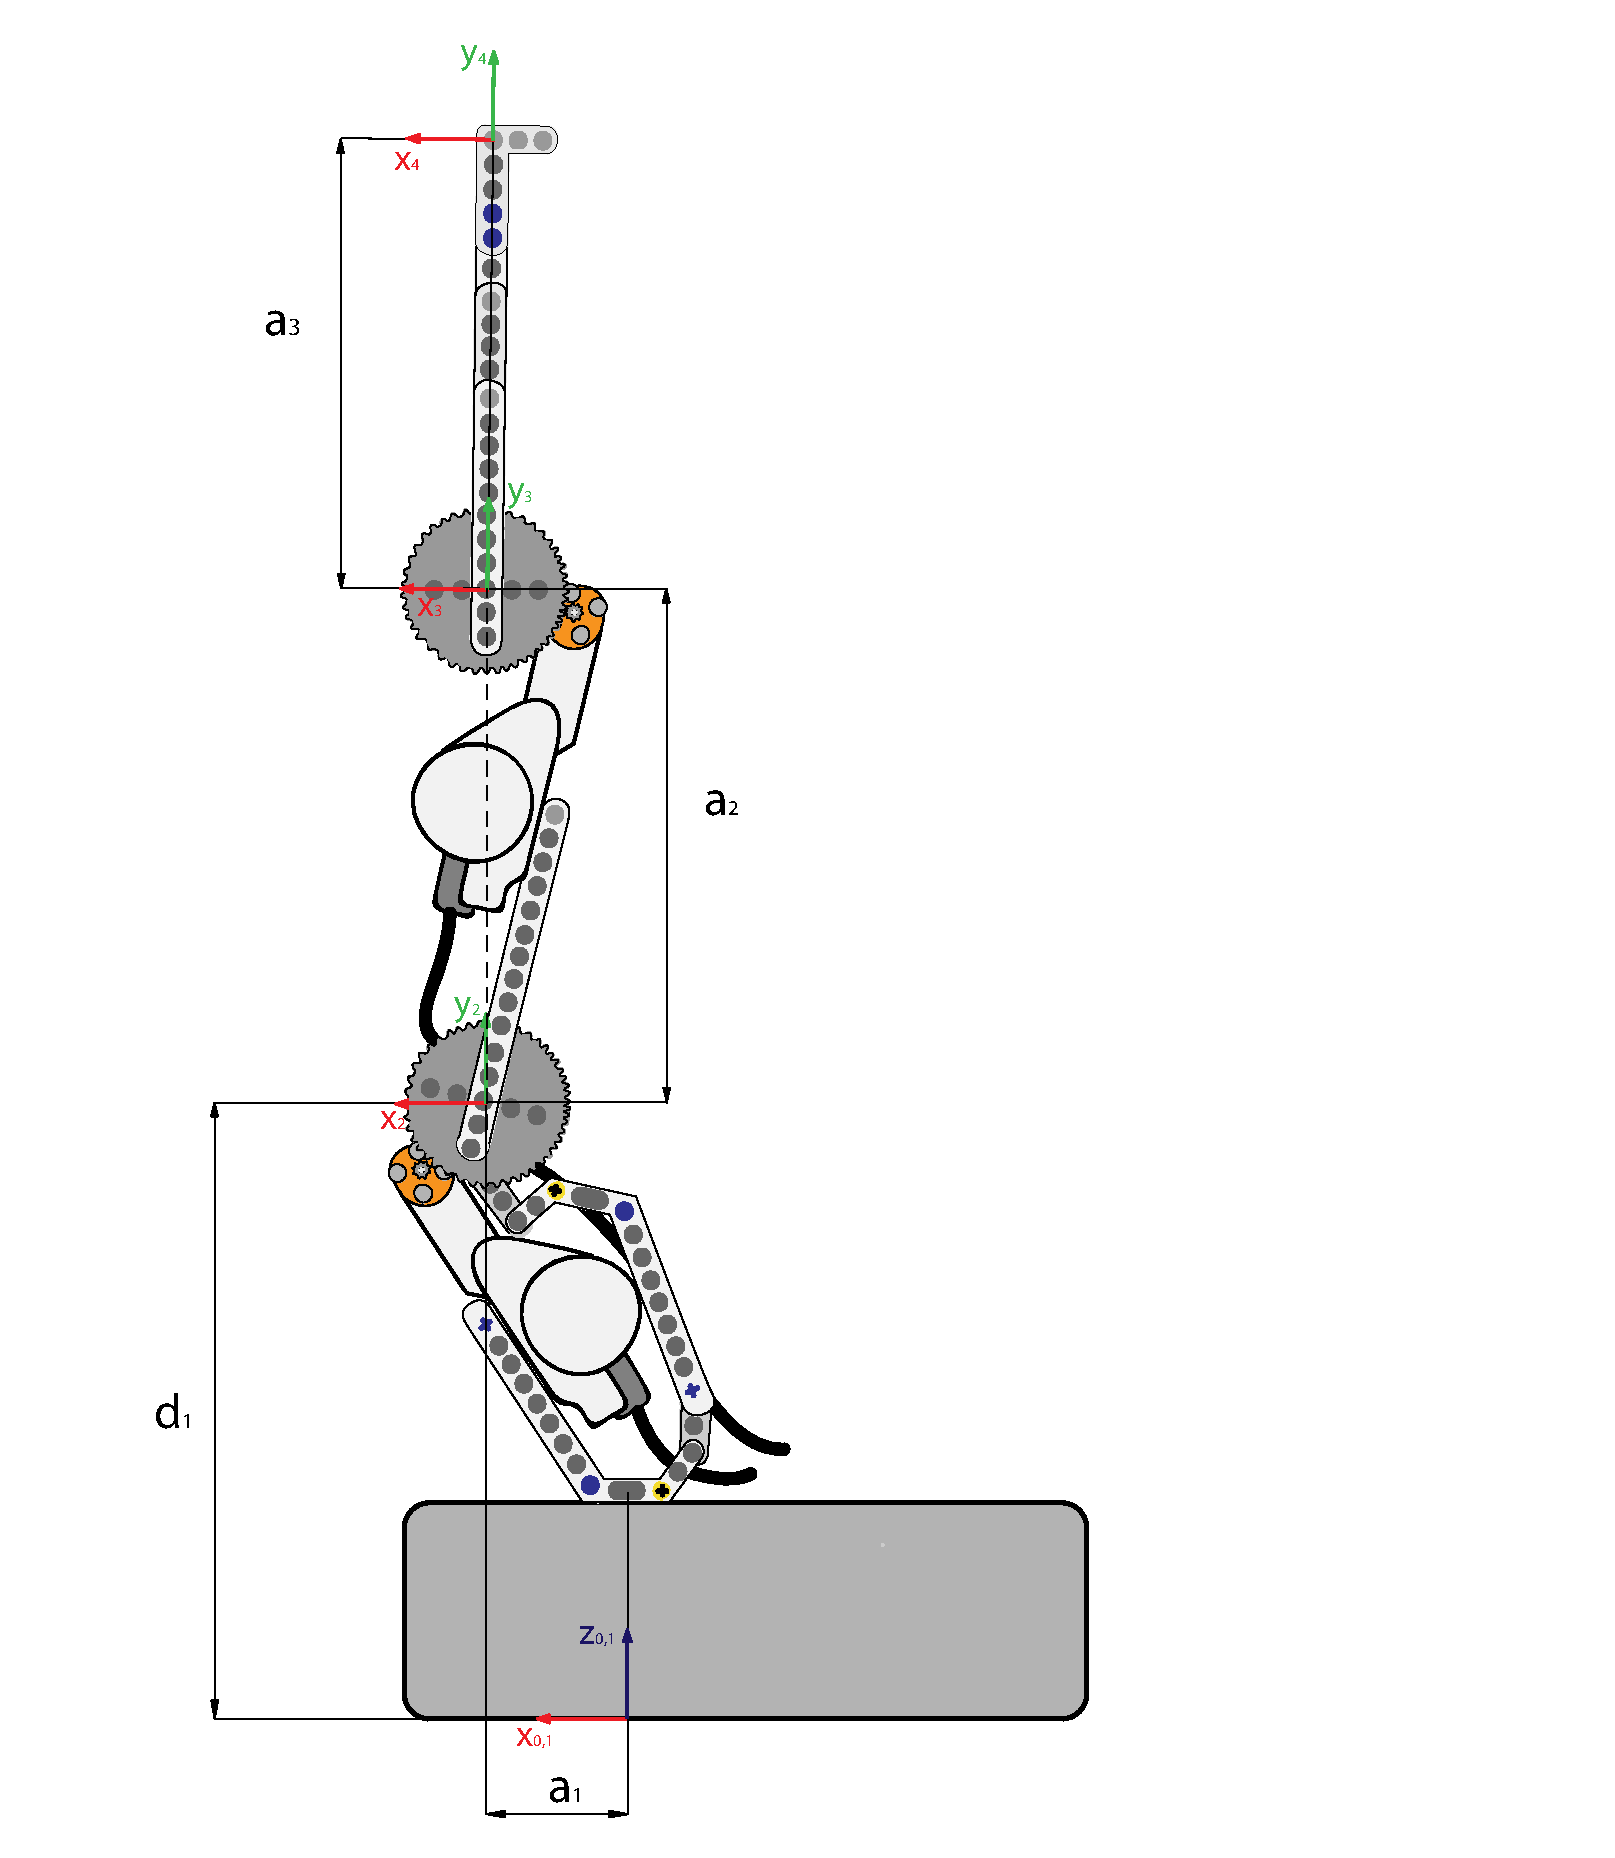
\includegraphics[width=0.575\textwidth]{DH2.pdf}\\
    Рисунок 2.1.3 Система с обозначенными DH параметрами.\\
\end{center}



\begin{table}[h!]
\hspace*{\parindent}Далее измеряются их значения и заносятся в соответствующую таблицу:\\
\begin{center}
\begin{tabular}{|c|c|c|c|c|}
\hline
Звено i & $a_i$ & $\alpha_i$ & $d_i$ & $\theta_i$ \\
\hline
1 & $a_1$ & $\frac{\pi}{2}$ & $d_1$ & $\theta_1$\\
\hline
2 & $a_2$ & 0 & $d_2$ & $\theta_2$ + $\frac{\pi}{2}$\\
\hline
3 & $a_3$ & 0 & $d_3$ & $\theta_3$\\
\hline
\end{tabular}
\end{center}
\end{table} 
\begin{center}
$a_1$ = 0,06 м;  $a_2$ = 0,15 м;  $a_3$ = 0,145 м; \\
$d_1$ = 0,163 м;  $d_2$ = 0 м;  $d_3$ = 0 м \\
\end{center}
\hspace*{\parindent}Подставив все параметры Денавита-Хартенберга для модели, представленной на рис.2.1.1, получим частный случай при n=3 матриц однородного преобразования:\\

\begin{equation*}\label{eq:model}
T_1^0 = 
     \begin{bmatrix}
    cos{\theta_1} & 0 &  -sin{\theta_1} & 0 \\
    sin{\theta_1} & 0 &  cos{\theta_1} & 0 \\
    0 & -1 & 0 & d_1\\
    0 & 0 & 0 & 1\\
    \end{bmatrix}
    ,
\end{equation*} 

\begin{equation*}\label{eq:model}
T_2^1 = 
     \begin{bmatrix}
    cos{(\theta_2 + \frac{\pi}{2})} & -sin{(\theta_2 + \frac{\pi}{2})} & 0 & a_2 cos{(\theta_2 + \frac{\pi}{2})} \\
    sin{(\theta_2 + \frac{\pi}{2})} & cos{(\theta_2 + \frac{\pi}{2})} & 0 & a_2 sin{(\theta_2 + \frac{\pi}{2})}\\
    0 & 0 & 1 & 0\\
    0 & 0 & 0 & 1\\
    \end{bmatrix}
    ,
\end{equation*} 

\begin{equation*}\label{eq:model}
T_3^2 = 
      \begin{bmatrix}
    cos{\theta_3 } & -sin{\theta_3} & 0 & a_3 cos{\theta_3} \\
    sin{\theta_3} & cos{\theta_3} & 0 & a_3 sin{\theta_3}\\
    0 & 0 & 1 & 0\\
    0 & 0 & 0 & 1\\
    \end{bmatrix}
    ,
\end{equation*}  
\end{document}


